\documentclass{ximera}
   
%% You can put user macros here
%% However, you cannot make new environments

\listfiles

\graphicspath{{./}{firstExample/}{secondExample/}}

\usepackage{tikz}
\usepackage{tkz-euclide}
\usepackage{tikz-3dplot}
\usepackage{tikz-cd}
\usetikzlibrary{shapes.geometric}
\usetikzlibrary{arrows}
\usetikzlibrary{decorations.pathmorphing,patterns}
\usetkzobj{all}
\pgfplotsset{compat=1.13} % prevents compile error.

\renewcommand{\vec}[1]{\mathbf{#1}}
\newcommand{\RR}{\mathbb{R}}
\newcommand{\dfn}{\textit}
\newcommand{\dotp}{\cdot}
\newcommand{\id}{\text{id}}
\newcommand\norm[1]{\left\lVert#1\right\rVert}
 
\newtheorem{general}{Generalization}
\newtheorem{initprob}{Exploration Problem}

\tikzstyle geometryDiagrams=[ultra thick,color=blue!50!black]

\usepackage{mathtools}
   
\title{Population Models Activity}
   
\begin{document}
   
\begin{abstract}
This activity demonstrates the wide ranging applicability of differential equation models in describing population trends.  Applications regarding the spread of disease and predator-prey relationships are explored in an interactive manner.  Students can manipulate key parameters in a model to optimize the fit to actual data.    
\end{abstract}
   
\maketitle
   
\section*{Overview of population models}
Differential equations are generally useful in predicting the time rate of change of any quantity.  Application topics vary widely, such as accounting for the changes in a system’s momentum, energy, or mass, describing the rate of production or destruction of a chemical in a reaction, or predicting how any type of population will evolve with time.  Consider any “Generic System” with a well-defined boundary that distinguishes between what is to be counted from everything else.  The quantity being counted could physically move in or out of the system at a certain rate.  If the quantity was the population of people in some country, these rates would correspond to rates of immigration and emigration.  In some systems, it is possible for the quantity to be generated or destroyed.  In a population example, these could be the birth and death rates.  These rates are depicted in the figure below, and tallied in an equation to describe the overall rate of accumulation of that quantity: 
 
 \begin{image}
 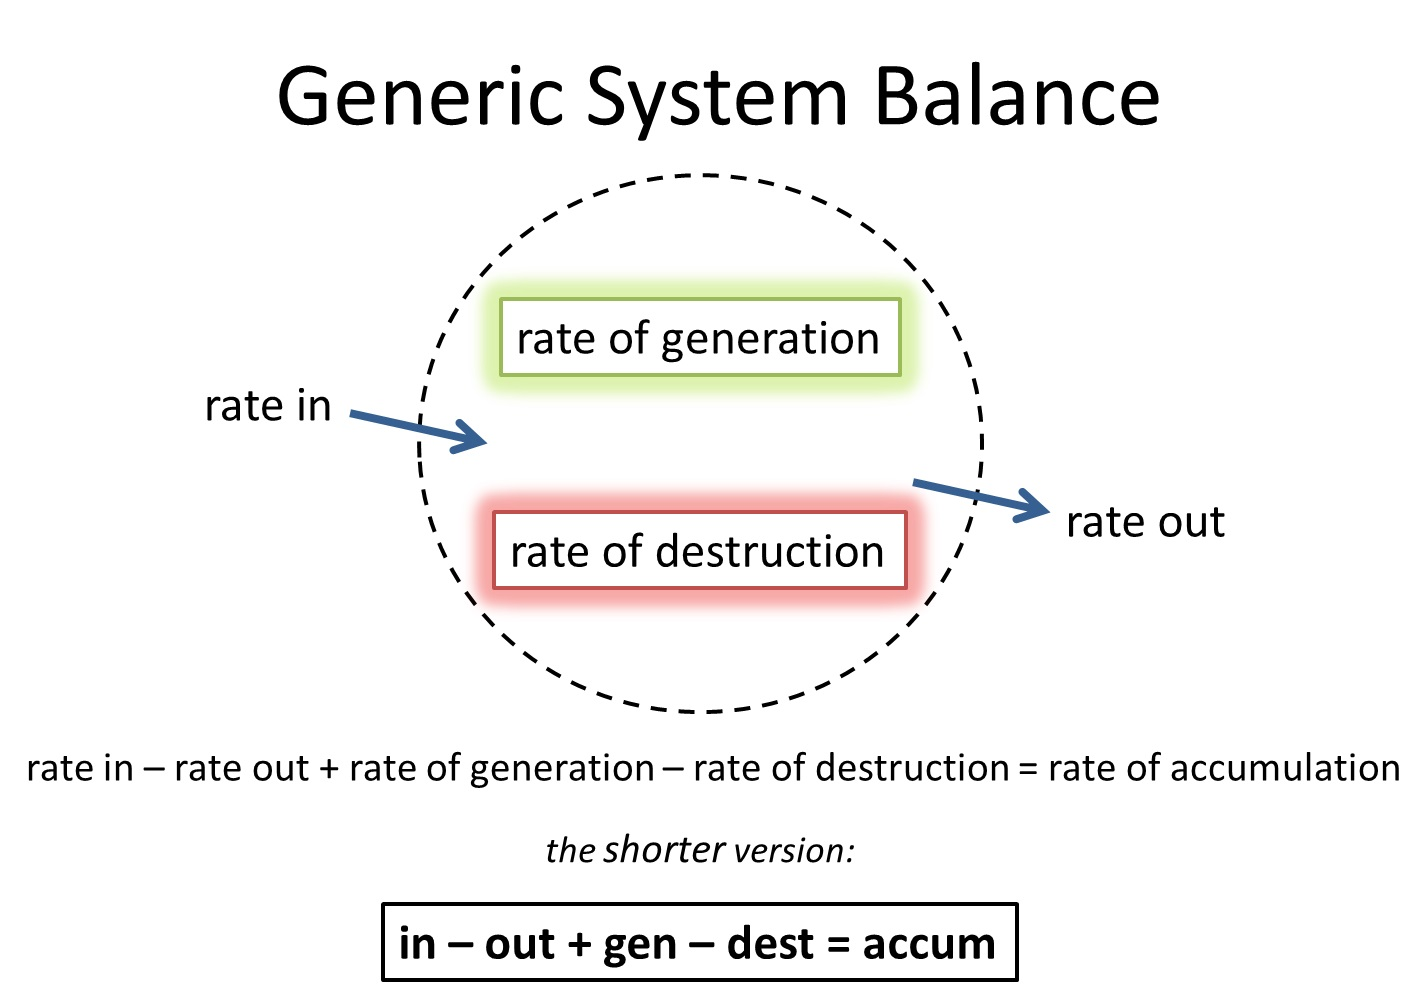
\includegraphics[height=1.5in]{population/populationModelPic.png} 
\end{image}

This concept quickly leads to a differential equation because the rate of accumulation is a first derivative of the quantity with respect to time.  In many interesting problems, some or all of the rates on the left hand side of the equation may depend on the quantity and/or time itself.  There are some physical quantities which are said to be ``conserved."  This means that -- under normal situations – they cannot be created or destroyed and those two terms would be zero.  These conserved quantities include mass, energy, momentum, and charge.  As noted above, a population of individuals is not generally conserved because birth and death may impact the population even in the absence of physical movement of individuals across the system boundary.  In a financial application such as modeling the amount of a given debt, more debt could be ``generated" through interest, which has a compounding effect over time.  Many other applications may begin with this concept of a generic system balance, but the examples below will especially focus on certain types of populations, whether human and animal.
 
\section*{Model of an Epidemic: The spread of a contagious but non-fatal disease} 

The spread of a disease in a community with a well-defined population is an interesting system in which to apply population modeling concepts with differential equations.  Certain diseases may not be fatal, and -- over time-scales of weeks or even months, there need not be any appreciable numbers of births or deaths in a given population.  Consider – for example – a documented outbreak of influenza at a boys' boarding school in England.  There were 763 boys in residence at the school.  The number of boys infected and confined to bed may be charted over time, providing a data set with which a model can be calibrated.  The table below contains information on the number of bedridden students among the total population of $N=763$ students.
$$ 
\begin{array}{|c|c|c|c|c|c|c|c|c|c|c|c|c|c|c|c|c|c|c|c|c|c|}\hline
\text{Time}           & 0 & 1 &  2 &  3 &  4 & 5 &   6  & 7 &   8 &   9 & 10 & 11 & 12 & 13  \\
\text{(in days)}&  &  &   &   &   &     &     &  &    &    &  &  &  & 
\\\hline
\text{Number of} &1 & 3 & 25 & 72 & 222 & 282 & 256 & 233 & 189 & 123 & 70 & 25 & 11 &  4 \\
\text{Bedridden} & &  &   &   &   &     &     &  &    &    &  &  &  & \\
\text{Boys} & &  &   &   &   &     &     &  &    &    &  &  &  & \\\hline
\end{array}
$$

We first enter the data using Sage lists, and plot the data:
 
\begin{sageCell}
days = srange(0, 14)
infected = [  1,   3,  25, 72, 222, 282, 256,
            233, 189, 123, 70,  25,  11,   4]
points(zip(days, infected))
\end{sageCell}

Only one of the 130 adult staff members at the school showed symptoms of the illness, so it is reasonable to ignore the adults in the model.  We begin by subdividing this total population into a susceptible population $S(t)$, an infected population $I(t)$, and a population of those recovered, $R(t)$.  Any one boy may progress from the susceptible, to the infected, and then to the recovered population as time progresses:
$$S(t)\longrightarrow I(t)\longrightarrow R(t)$$
The first step in this process represents infection and the second step represents recovery.  If we propose that those boys recovered from the flu are now immune to that strain, the illness only affects each boy at-most once.  Only one of the boys may have originally been infected with the disease, giving the following initial conditions:
$$S(0)=762,\quad I(0)=1,\quad R(0)=0$$
Differential equations could be written to account for the change in all three of these sub-populations, but, in practice, it will only be necessary to model two of these because the total population of 763 is constant:
$$S+I+R=763$$
We must consider every way in which the population of a particular sub-population could change.  Considering the generic system balance above, we might visualize boys ``moving" from one sub-population to the next.  To model the change in the number of boys infected with the flu, we need to account for the processes of infection and recovery.  These rates will tend to increase and decrease the number of infected boys, respectively.  Let's assume that the boys at the school encounter one another randomly and that a fixed proportion of these random encounters between an infected boy and a healthy boy that is susceptible results in a new infection.  If we also assume a constant relative recovery rate from the flu for those who are infected, the following differential equation may be proposed:
$$\frac{dI}{dt}=kIS-rI $$
The differential equation tells us how the number of infected boys will change with time.  The associated units of this rate equation are boys/day.  Here, $k$ is a constant of proportionality that incorporates the random rate of encounters which may lead to new infections.  The units of $k$ are 1/(boys)(day).  The units of the relative recovery rate $r$ are 1/day.  This relative rate of recovery is the only contributing factor increasing the number of boys who are recovered, so the differential equation for the number of recovered boys is simply:
$$\frac{dR}{dt}=rI $$
It is not necessary to directly model the population of susceptible boys, as that can be written in terms of the total number and the other two sub-populations:
$$S=763-I-R$$
This allows us to modify the first differential equation, replacing $S$
$$\frac{dI}{dt}=kI(763-I-R)-rI$$
The two differential equations describing the changes in $I$ and $R$ may now be solved with initial conditions.  Initially, 762 boys are susceptible, one boy is infected because he caught the flu over break, and no boys are yet recovered:
$$I(0)=1,\quad R(0)=0$$
The next Sage cell demonstrates how to solve the system of differential equations for the following values of the parameters:
\[
r = 0.5206,\quad k = 0.0473,\quad p = 0.07
\]
and the initial conditions:
\[
I(0)=1,\quad R(0)=0:
\]
 
\begin{sageCell}
I, R = var('I R')
r = 0.5206
k = 0.0473
p = 0.07
N = 763
desyst = [p*k*I*(N-I-R) - r*I, r*I]
ics = [1, 0]
tvalues = srange(0.0, 13.0, 0.1)
soln = desolve_odeint(desyst, ics, tvalues, [I, R])
g = points(zip(days, infected),size=48, color='red')
g += line(zip(tvalues, soln[:,0]),color='blue')
g.show()\end{sageCell}
 
Click the $\mathtt{Evaluate}$ button to compute the solution and plot the solution.
 
To fit the model to the data, we would like to find the values of the parameters that minimize the sum of squared errors. Use the sliders in the interactive display below to try to guess what are the optimal values of $k$ and $r$, where we assume that $p=0.07$:
 
\begin{sageOutput}
days = srange(0, 14)
infected = [  1,   3,  25, 72, 222, 282, 256,
            233, 189, 123, 70,  25,  11,   4]
I, R = var('I R')
NPop = 763
@interact
def _(r=slider(0,1,0.01,0.01),
      k=slider(0,0.2,0.001,0.01)):
    p = 0.07
    N = 763   
    ics = [1.0, 0.0]
    desyst = [p*k*I*(N-I-R) - r*I, r*I]
    tvalues = srange(0.0, 13.0, 0.1)
    soln = desolve_odeint(desyst, ics, tvalues, [I, R])
    g = points(zip(days, infected), size=48, color='red')
    g += line(zip(tvalues, soln[:,0]), color='blue')
    g.show(xmin=0, xmax=13, ymin=0, ymax=300)
    soln = desolve_odeint(desyst, ics, days, [I, R])
    Ivalues = soln[:,0]
    sse = sum((infected-Ivalues)^2)
    pretty_print(html('Sum of squared errors: {}'.format(sse)))
\end{sageOutput}

\begin{problem}
The values that minimize the sum of squared errors are:
 
$r=\answer{0.49}$
 
$k=\answer{0.037}$
\end{problem}

\section*{Predator-Prey Model with Lynx and Snowshoe Hares}

Another important application of differential equations in modeling population concerns predator-prey dynamics.  In systems where two species -- the predator and prey -- are the primary sources of predation and food for one another, respectively.  In these cases their populations are closely linked.  A growth in predator population causes a decrease in the population of prey, a trend which reverses when the predator population ultimately decreases when less food is available.  Examples include cheetah and gazelle, osprey and fish (as a general grouping of species), and blue whales and krill.  The example we will consider here is the Canadian lynx and snowshoe hare populations.  This is a classic and well-studied example because of the many decades of data compiled by trappers working for The Hudson’s Bay Company.  Periodic fluctuations in both populations were recorded over 90 years:

%insert graph of data below in Ximera with Sage code

While more advanced models of predator-prey relationships have been proposed, the differential equations commonly employed here are called the Lotka-Volterra equations, named for the scientists who developed them independently.  They are a pair of non-linear differential equations that contain four parameters that may be adjusted for different systems.  To model, the population of hare ($h$) and the population of lynx ($l$), these are:
$$\frac{dh}{dt}=ah-bhl,\quad\frac{dl}{dt}=-ml+nhl$$
The parameter a in the hare equation is the relative rate of growth of hare without any predation by the lynx.  If the lynx population, which appears in the second term ($bhl$) were zero, then the hare population would simply grow exponentially (at a rate proportional to its size).  This second term captures the actual effect of predation, which reduces the hare population at a rate proportional to the hare and lynx population.  This constant of proportionality is $b$.  The second equation, modeling the lynx population, includes a term to account for the relative death rate m of lynx if no hares were present as their food.  The parameter n in the second term is the constant of proportionality specifying the growth of lynx due to their predation of hares.  Just as the decrease in hares due to predation is proportional to the product of predator and prey populations, so too is the increase in lynx.  Many implicit assumptions are made in formulating this model.  It is assumed that the population of snowshoe hares is limitless in the absence of the lynx and that the appetite of the lynx is limitless even with very large populations of hares.  We are essentially assuming that the prey is not limited in any fundamental way by its own food (plant) population, or other resources including space.  Another key assumption that is never entirely true is that the predator is the only source of attack on the prey population and that the prey is the only source of food for the predator.  In spite of their obvious importance, outside environmental factors, seasonal dynamics, and impacts by other species including humans -- such as by trapping -- are ignored.  More complicated approaches could account for the actual limits to both populations (through a logistic model), the limits to the predation capacity of the lynx, and any other predator-prey dynamics with other species (such as between the snowshoe hare and its various plant food sources).  Nevertheless, the Lotka-Volterra equations have sufficient predictive power for us to adjust these parameters and make a rudimentary fit to the recorded data.
Initial conditions for the lynx and hare populations are taken directly from the first available data beginning in 1845:
$$h(0)=20,\quad l(0)=36$$
Here again, SageMath code numerically solves the system of differential equations given values for the four parameters:

%need sage code

\section*{Sources}
Influenza in a boarding school (1978 British Medical Journal): 

\href{http://www.ncbi.nlm.nih.gov/pmc/articles/PMC1603269/pdf/brmedj00115-0064.pdf}{http://www.ncbi.nlm.nih.gov/pmc/articles/PMC1603269/pdf/brmedj00115-0064.pdf}

SIMIODE Example 6-1-S-Epidemic, MODELING A NONLETHAL INFLUENZA EPIDEMIC, Sheila Miller, Department of Mathematics, New York City College of Technology City University of New York Brooklyn NY USA. 

\href{https://www.simiode.org/resources/572}{https://www.simiode.org/resources/572}
\end{document}